\section{Auswertung}

\subsection{Leerlaufspannung und Eigenwiderstand (Messung a)}
Das Voltmeter hat einen Eingangswiderstand von
\begin{equation}
	R_\text{v} \ge 10 \text{M \Omega} \notag
\end{equation}.
Die Leerlaufspannung beträgt:
\begin{equation}
	U_\text{0,Mono} = \SI{1.6}{V} \notag
\end{equation}

\subsection{Klemmenspannung an Monozelle (Messung b)}
Die gemessenen Werte sind in Tabelle \ref{tab:b} abzulesen.

\begin{table}[h!]
    \begin{center}
      \caption{Messung der Klemmenspannung an einer Monozelle (Messung b).}
      \label{tab:b}
      \begin{tabular}{c|c} 
        \textbf{$I / mA$} & \textbf{$U_k / V$}\\
        \hline
		88 & 0,15 \\
		69 & 0,48 \\
		56 & 0,70 \\
		47 & 0,85 \\
		40 & 0,96 \\
		36 & 1,10 \\
		32 & 1,20 \\
		29 & 1,25 \\
		27 & 1,30 \\
		24 & 1,31 \\
		23 & 1,40 \\
      \end{tabular}
    \end{center}
\end{table}
Aus diesen Werten lassen sich nun der Innenwiderstand und die Leerlaufspannung der Monozelle bestimmen.
Dazu wird die allgemeine Geradengleichung verwendet.
\begin{equation}
    y = m \cdot x + b
\end{equation}
Aus den gemessen Werten und der linearen Regression ergeben sich jeweils Werte für die Steiung $m$ und den Achsenabschnitt $b$.
Dabei entspricht die Steigung der Geraden dem Innenwiderstand $R_i$, wie aus Gleichung (5) erkennbar wird, und der Achsenabschnitt der Leerlaufspannung $U_0$.

\begin{figure}[h]
  \centering
  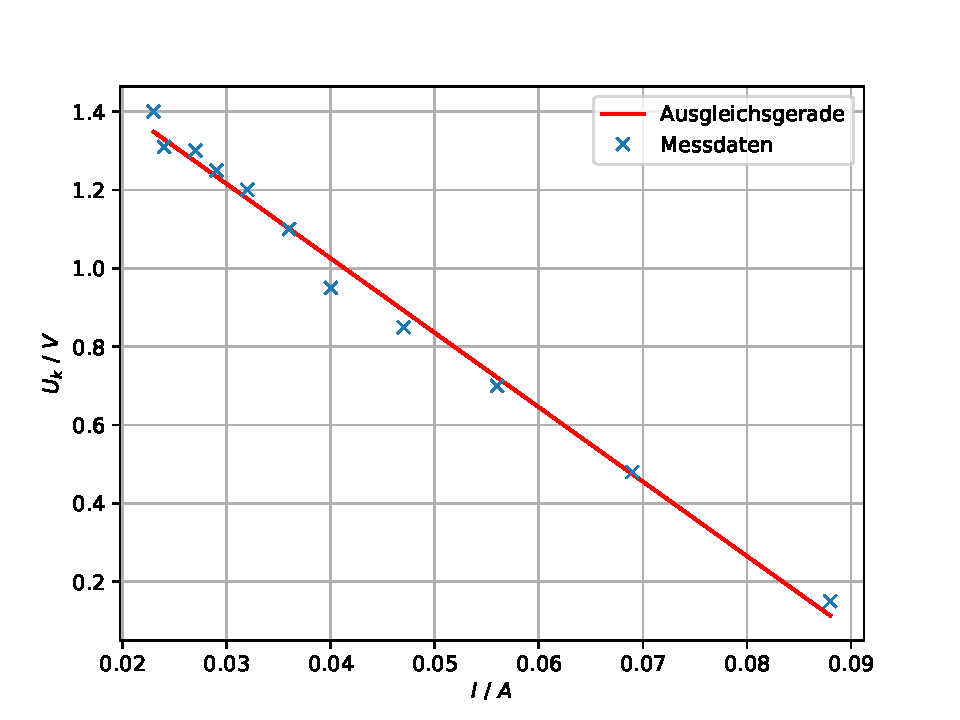
\includegraphics[height=8cm]{Auswertung/B_Innenwiderstand.pdf}
  \caption{Innenwiderstand der Monozelle aus b).}
  \label{fig:B_Innenwiderstand.pdf}
\end{figure}

\begin{equation}
    |m_1| = R_i = \SI{18,998 \pm 0,360}{\Omega} \notag
\end{equation}
\begin{equation}
    b_1 = U_0 = \SI{1,785 \pm 0,0008}{V} \notag
\end{equation}
\newpage
Bei der Methode der Gegenspannung ergeben sich die in der \ref{tab:c} aufgetragenen Werte.
\begin{table}[h!]
    \begin{center}
      \caption{Methode der Gegenspannung (Messung c).}
      \label{tab:c}
      \begin{tabular}{c|c} 
        \textbf{$I / mA$} & \textbf{$U_k / V$}\\
        \hline
		120 & 4,00 \\
		90 & 3,50 \\
		74 & 3,20 \\
		63 & 3,00 \\
		57 & 2,90 \\
		54 & 2,80 \\
		50 & 2,70 \\
		45 & 2,60 \\
		43 & 2,60 \\
		35 & 2,45 \\
		31 & 2,40 \\
      \end{tabular}
    \end{center}
\end{table}

Dort wird ebenfalls nach (6) die lineare Regression angewendet, um die Leerlaufspannung $U_0$ und den Innenwiderstand $R_i$ zu bestimmen.
Dabei ergeben sich folgende Werte.

\begin{equation}
    m_2 = R_i = \SI{18,508 \pm 0,119}{\Omega} \notag
\end{equation}
\begin{equation}
    b_2 = U_0 = \SI{1,809 \pm 0,0005}{V} \notag
\end{equation}

\begin{figure}[h]
  \centering
  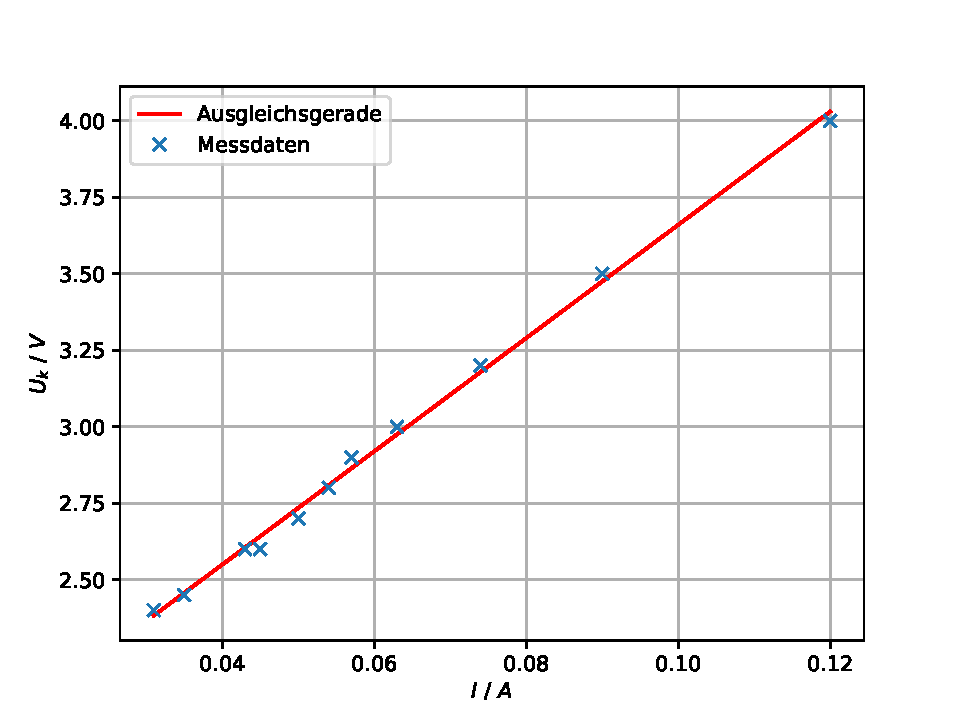
\includegraphics[height=8cm]{Auswertung/C_Innenwiderstand.pdf}
  \caption{Innenwiderstand der Monozelle aus c).}
  \label{fig:C_Innenwiderstand.pdf}
\end{figure}

Bei der Messung mit der Rechtecks- und Sinusspannung ergeben sich die Werte aus \ref{tab:d}.
\begin{table}[h!]
    \begin{center}
      \caption{Rechtecks- und Sinusspannung(Messung d).}
      \label{tab:d}
      \begin{tabular}{c|c|c|c} 
        \textbf{$I / mA$} & \textbf{$U_k / V$} & \textbf{$I / mA$} &  \textbf{$U_k / V$}\\
        \hline
        7,0 & 0,175 & 22,0 & 6,0\\
		6,2 & 0,210 & 22,0 & 6,2\\
		5,5 & 0,250 & 21,0 & 6,5\\
		5,2 & 0,270 & 19,0 & 7,1\\
		4,6 & 0,280 & 17,5 & 7,5\\
		4,1 & 0,310 & 16,0 & 7,9\\
		3,7 & 0,330 & 10,5 & 8,7\\
		3,3 & 0,360 & 8,0 & 9,1\\
        3,0 & 0,380 & 3,0 & 9,8\\
        2,6 & 0,390 & 2,8 & 9,9\\
      \end{tabular}
    \end{center}
\end{table}

Für die Rechtecksspannung lassen sich folgende Werte durch (6) und die lineare Regression bestimmen.
\begin{equation}
    |m_3| = R_i = \SI{49,381 \pm 3,355}{\Omega} \notag
\end{equation}
\begin{equation}
    b_3 = U_0 = \SI{519,201 \pm 0,075}{mV} \notag
\end{equation}

\begin{figure}[h]
  \centering
  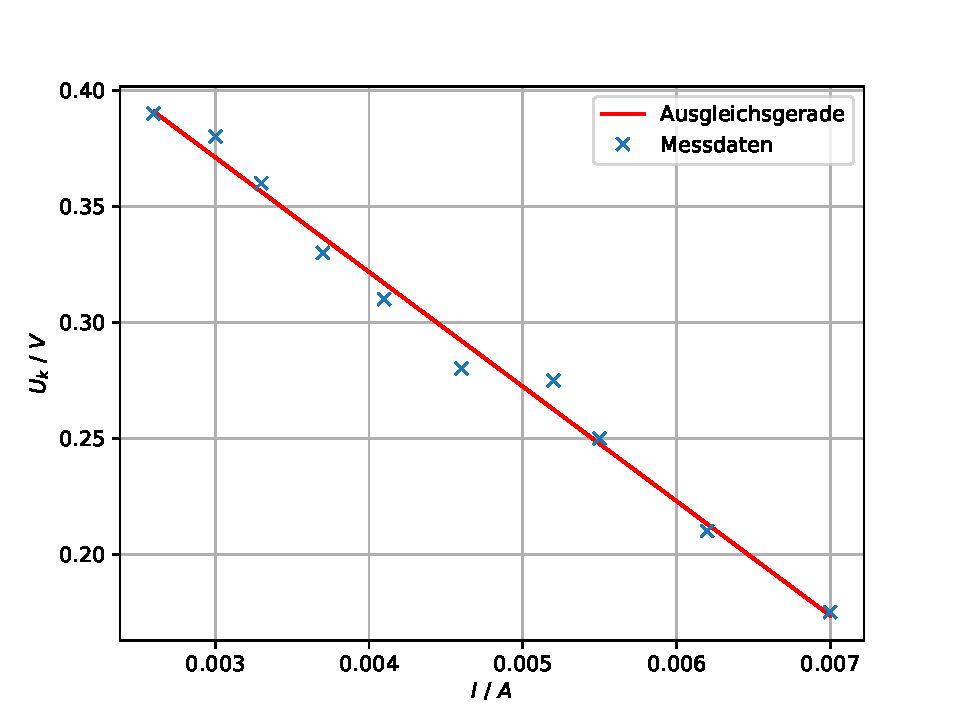
\includegraphics[height=8cm]{Auswertung/Rechteck.pdf}
  \caption{Verlauf der Rechteckspannung aus d).}
  \label{fig:Rechteck.pdf}
\end{figure}

Bei der Sinusspannung ergeben sich mit der gleichen Methode folgende Werte:
\begin{equation}
    |m_4| = R_i = \SI{189,705 \pm 120,196}{\Omega} \notag
\end{equation}
\begin{equation}
    b_4 = U_0 = \SI{10,560 \pm 0,030}{V} \notag
\end{equation}

\begin{figure}[h]
  \centering
  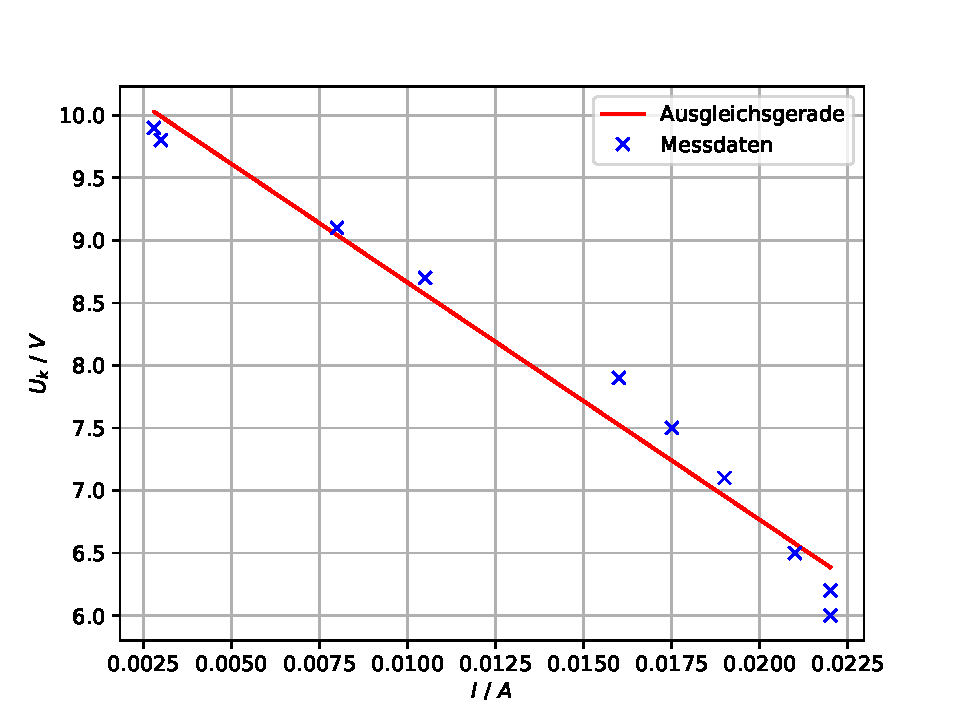
\includegraphics[height=8cm]{Auswertung/Sinusspannung.pdf}
  \caption{Verlauf der Sinusspannung aus d).}
  \label{fig:Sinusspannung.pdf}
\end{figure}

\subsection{Systematische Fehler bei der $U_0$-Messung}
Der systematische Fehler bei der Berechnung für die Leerlaufspannung $U_0$ wird über die Beziehungen in einer Reihenschaltung und die Kirchhoffschen Regeln bestimmt.
Der Fehler kommt aufgrund des endlichen Widerstandes $R_V$ des Voltmeters zustande.
\begin{equation}
    U_0 = I \cdot R_\text{ges} = I \cdot (R_V + R_i) = \frac{U_k}{R_V} \cdot (R_V + R_i) = U_k \left(1+\frac{R_i}{R_V}\right)  \notag
\end{equation}
Aus dem Verhältnis $U_0/U_k$ kann der relative Fehler auf $1,8998 \cdot 10^{-6}$ bestimmt werden.
Der absolute Fehler beträgt
\begin{equation}
    \Delta U_0 = U_\text{0,exp} \frac{R_i}{R_V} = \SI{3,04}{\cdot}{10^{-6}}{V}    \notag
\end{equation}

\subsection{Systematischer Fehler bei nachgeschaltetem Voltmeter}
Falls das Voltmeter hinter das Amperemeter geschaltet wird, kommt bei einem realen Amperemeter dessen Eigenwiderstand noch dazu.
Bei einem idealen Amperemeter ist dieser Eigenwiderstand gleich null.
In der Realität wird der Eigenwiderstand möglichst klein gehalten, aber verschwindet nicht.
Dadurch ergibt sich für den systematischen Fehler Folgendes:
\begin{equation}
    \Delta U_0 = U_\text{0,exp} \left (\frac{R_i}{R_V} + \frac{R_A}{R_V} \right)  \notag
\end{equation}

\subsection{Umgesetzte Leistung}
In der Tabelle \ref{tab:e} werden die Werte aus der ersten Messung und zusätzlich der Belastungswiderstand $R_a$ und die Leistung $N$ nach (4) bestimmt.
Das Diagramm zeigt die Abhängigkeit der Leistung vom Widerstand in der Theorie und im Experiment.
Dabei errechnet sich die theoretische Kurve nach (4) folgendermaßen.
\begin{equation}
    N_\text{theo} = I^{2} R_a = \left (\frac{U_0}{R_i+R_a} \right )^{2} \cdot R_a
\end{equation}
\begin{table}[h!]
    \begin{center}
      \caption{Umgesetzte Leistung.}
      \label{tab:e}
      \begin{tabular}{c|c|c|c} 
        \multicolumn{2}{c|}{Rechteckspannung} & \multicolumn{2}{c}{Sinusspannung} \\
        \hline
        \textbf{$I / mA$} & \textbf{$U_k / V$} & \textbf{$R_a / \Omega$} &  \textbf{$N / mW$}\\
        \hline
		88 & 0,15 & 1,71 & 13,2\\
		69 & 0,48 & 6,96 & 33,1\\
		56 & 0,70 & 12,50 & 39,2\\
		47 & 0,85 & 18,09 & 40,0\\
		40 & 0,96 & 23,75 & 38,0\\
		36 & 1,10 & 30,56 & 39,6\\
		32 & 1,20 & 37,50 & 38,4\\
		29 & 1,25 & 43,10 & 36,3\\
		27 & 1,30 & 48,15 & 35,1\\
		24 & 1,31 & 54,58 & 31,4\\
		23 & 1,40 & 60,87 & 32,2\\
      \end{tabular}
    \end{center}
\end{table}

\begin{figure}[h!]
  \centering
  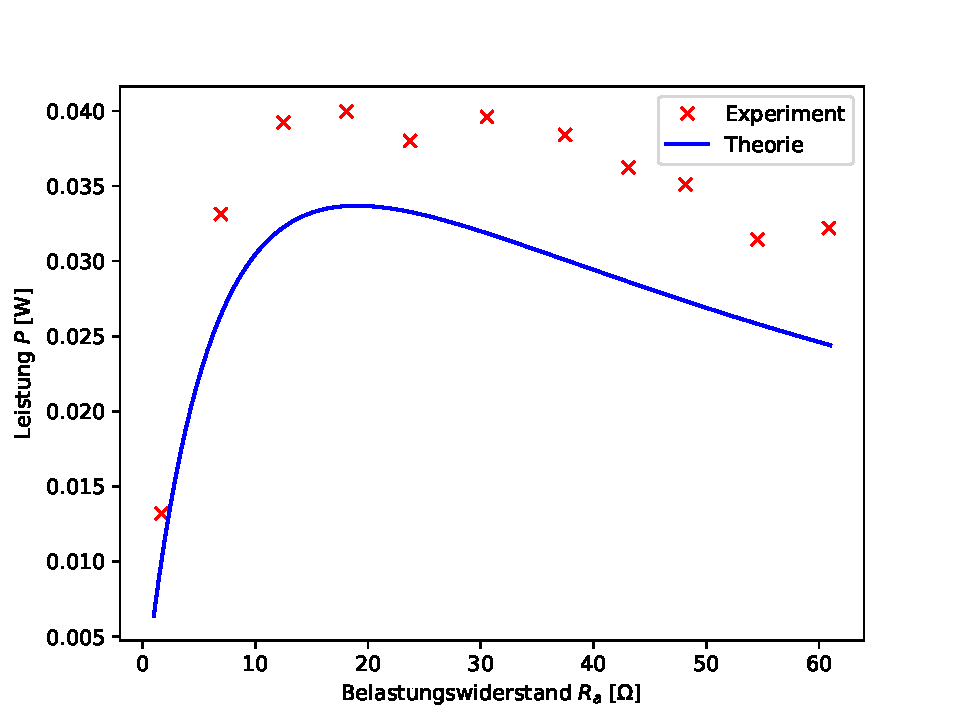
\includegraphics[height=8cm]{Auswertung/Leistung.pdf}
  \caption{Verlauf der umgesetzten Leistung.}
  \label{fig:Leistung.pdf}
\end{figure}

\newpage
